\chapter[Общие сведения о языке \Sys{С++}]{Общие сведения о языке \Sys{С++}}\label{gl02}
В этой главе читатель познакомится с основными элементами языка \Sys{С++}: алфавитом, переменными, константами, типами данных,
основными операциями, стандартными функциями, структурой программы и средствами ввода вывода данных.

\section[Алфавит языка]{Алфавит языка}
Программа на языке \Sys{С++} может содержать следующие символы:
\begin{itemize}
\item прописные, строчные латинские буквы A, B, C, …, x, y, z и знак подчеркивания;
\item арабские цифры от 0 до 9;
\item специальные знаки: “ \{ \} , {\textbar} [ ] ( ) + --- / \% * . {\textbackslash} ‘ : ? {\textless} = {\textgreater} !
\& \# \~{} ; \^{}
\item символы пробела, табуляции и перехода на новую строку.
\end{itemize}
Из символов алфавита формируют ключевые слова и идентификаторы. \index{Ключевые слова}{Ключевые слова}
 --- это зарезервированные слова, которые имеют специальное значение для компилятора и используются только в том смысле, в
котором они определены (операторы языка, типы данных и т.п.). \index{Идентификатор}Идентификатор ---
это имя программного объекта, представляющее собой совокупность букв, цифр и символа подчеркивания. Первый символ
идентификатора --- буква или знак подчеркивания, но не цифра. Идентификатор не может содержать пробел. Прописные и
строчные буквы в именах различаются, например, \Sys{ABC}, \Sys{abc}, \Sys{Abc} --- 
три различных имени. Каждое имя (идентификатор) должно быть уникальным в пределах функции и не совпадать с ключевыми
словами. 

В тексте программы можно использовать \index{Комментарии}комментарии. Если текст начинается с двух
символов «косая черта» // и заканчивается символом перехода на новую строку или заключен между
символами /* и */, то компилятор его игнорирует. 

\begin{lstlisting}
/* `\Sys{Комментарий может}`
 `\Sys{выглядеть так!}`*/
//`А если вы используете такой способ,`
//`то каждая строка должна начинаться`
//`с двух символов «косая черта».`
\end{lstlisting}
Комментарии удобно использовать как для пояснений к программе, так и для временного исключения фрагментов программы при
отладке.

\section[Данные]{Данные}
Для решения задачи в любой программе выполняется обработка каких-либо данных. Данные хранятся в памяти компьютера и
могут быть самых различных типов: целыми и вещественными числами, символами, строками, массивами. \index{Типы
данных}{Типы данных} определяют способ хранения чисел или символов в памяти компьютера. Они задают
размер ячейки, в которую будет записано то или иное значение, определяя тем самым его максимальную величину или
точность задания. Участок памяти (ячейка), в котором хранится значение определенного типа, называется
\index{Переменная}переменной. У переменной есть \index{Переменная!имя}имя
(идентификатор) и \index{Переменная!значение}значение. Имя служит для обращения к области памяти, в
которой хранится значение. Во время выполнения программы значение переменной можно изменить. Перед использованием любая
переменная должна быть описана. \index{Переменная!описание}Оператор описания переменных в языке \Sys{С++}
имеет вид:
\begin{itemize}
\item[] \Sys{тип имя\_переменной;}
\end{itemize}
или
\begin{itemize}
\item[] \Sys{тип список\_переменных;}
\end{itemize}

Типы данных языка \Sys{С++} можно разделить на основные и составные.

К \index{Типы данных!основные}основным типам данных языка относят:
\begin{itemize}
\item \Sys{char} --- символьный; 
\item \Sys{int} --- целый; 
\item \Sys{float} --- с плавающей точкой; 
\item \Sys{double} --- двойной точности; 
\item \Sys{bool} --- логический.
\end{itemize}
Для формирования других типов данных используют основные типы и так называемые спецификаторы. Типы данных, созданные на
базе стандартных типов с использованием спецификаторов, называют \index{Типы данных!составные}составными типами данных. 
В \Sys{С++} определены четыре спецификатора типов данных:
\begin{itemize}
\item \Sys{short} --- короткий;
\item \Sys{long} --- длинный;
\item \Sys{signed} --- знаковый;
\item \Sys{unsigned} --- беззнаковый.
\end{itemize}
Далее будут рассмотрены назначение и описание каждого типа.

\subsection[Символьный тип]{Символьный тип}
Данные типа \Sys{char} в памяти компьютера всегда занимают один байт\footnote{В кодировке utf каждый символ
кириллицы занимает 2 байта.}. Это связано с тем, что обычно под величину символьного типа отводят столько памяти,
сколько необходимо для хранения любого из 256 символов клавиатуры. \index{Типы данных!символьный}Символьный тип может
быть со знаком или без знака (табл. \ref{ch02:refTable0}).

\noindent
\begin{longtable}{|l|r|r|}
\caption{Символьные типы данных} \label{ch02:refTable0}\\
\hline
\Emph{Тип}&\Emph{Диапазон}&\Emph{Размер}\\ 
\hline \hline 
\endfirsthead
\multicolumn{3}{c}%
{{\tablename\ \thetable{} --- продолжение}} \\
\hline
\Emph{Тип}&\Emph{Диапазон}&\Emph{Размер}\\ 
\hline \hline
\endhead
\Sys{char} & –128…127 & 1 байт\\\hline
\Sys{unsigned char} & 0…255 &1 байт\\\hline
\Sys{signed char} &–128…127 &1 байт\\\hline
\end{longtable}

Пример описания символьных переменных:

\Sys{char c, str; //Описаны две символьные переменные.}

При работе с символьными данными нужно помнить, что если в выражении встречается одиночный символ, он должен быть
заключен в одинарные кавычки. Например, \Sys{'a'}, \Sys{'b'}, \Sys{'+'},
\Sys{'3'}.

Последовательность символов, то есть строка, при использовании в выражениях заключается в двойные кавычки:
\Sys{”Hello!”}.

\subsection[Целочисленный тип]{Целочисленный тип}
Переменная типа \Sys{int} в памяти компьютера может занимать либо два, либо четыре байта. Это зависит от
разрядности процессора. 

Диапазоны значений \index{Типы данных!целый}целого типа представлены в таблице \ref{ch02:refTable1}. По умолчанию все
целые типы считаются знаковыми, т.е. спецификатор \Sys{signed} можно не указывать.


\noindent
\begin{longtable}{|l|c|l|}
\caption{Целые типы данных} \label{ch02:refTable1}\\
\hline
\Emph{Тип}&\Emph{Диапазон}&\Emph{Размер}\\
\hline \hline
\endfirsthead
\multicolumn{3}{c}%
{{\tablename\ \thetable{} --- продолжение}} \\
\hline
\Emph{Тип}&\Emph{Диапазон}&\Emph{Размер}\\
\hline \hline
\endhead
\Sys{int} &–2147483647 …  2147483647 &4 байта\\\hline
\Sys{unsigned int} &0 … 4294967295 &4 байта\\\hline
\Sys{signed int} &–2147483647 …  2147483647 &4 байта\\\hline
\Sys{short int} &–32767 … 32767 &2 байта\\\hline
\Sys{long int} &–2147483647 … 2147483647 &4 байта\\\hline
\Sys{unsigned short int} &0 … 65535 &2 байта\\\hline
\Sys{signed short int} &–32767 … 32767 &2 байта\\\hline
\Sys{long long int} &–($2^{63}$–1) … ($2^{63}$–1) &8 байт\\\hline
\Sys{signed long int} & –2147483647 … 2147483647 &4 байта\\\hline
\Sys{unsigned long int} &0 … 4294967295 &4 байта\\\hline
\Sys{unsigned long long int} &0 … ${2^{64}}$–1  &8 байт\\\hline
\end{longtable}

Пример описания целочисленных данных:

\Sys{int a, b, c;}

\Sys{unsigned long int A, B, C;}

\subsection[Вещественный тип]{Вещественный тип}
Внутреннее представление \index{Типы данных!вещественный}вещественного числа в памяти компьютера отличается от
представления целого числа. Число с плавающей точкой представлено в  экспоненциальной форме
$mE\pm p$, где $m$ --- мантисса (целое или дробное число с
десятичной точкой), $p$ --- порядок (целое число). Для того чтобы перевести число в экспоненциальной
форме к обычному представлению с фиксированной точкой, необходимо мантиссу умножить на десять в степени порядок.
Например, 

 $-6.42E+2=-6.42\cdot 10^{2}=-642$,

$3.2E-6=3.2\cdot 10^{-6}=0.0000032$

Обычно величины типа \Sys{float} занимают 4 байта, из которых один двоичный разряд отводится под знак, 8
разрядов под порядок и 23 под мантиссу. Поскольку старшая цифра мантиссы всегда равна 1, она не хранится.

Величины типа \Sys{double} занимают 8 байт, в них под порядок и мантиссу отводится 11 и 52 разряда
соответственно. Длина мантиссы определяет точность числа, а дли-на порядка его диапазон. Спецификатор типа
\Sys{long} перед именем типа \Sys{double} указывает, что под величину отводится 10 байт.

Диапазоны значений вещественного типа представлены в таблице~\ref{ch02:refTable2}.


\noindent
\begin{longtable}{|l|c|l|}
\caption{Вещественные типы данных} \label{ch02:refTable2}\\
\hline
\Emph{Тип}&\Emph{Диапазон}&\Emph{Размер}\\
\hline \hline
\endfirsthead
\multicolumn{3}{c}%
{{\tablename\ \thetable{} --- продолжение}} \\
\hline
\Emph{Тип}&\Emph{Диапазон}&\Emph{Размер}\\
\hline \hline
\endhead
\Sys{float} &3.4Е-38 … 3.4E+38 &4 байта\\\hline
\Sys{double} &1.7Е-308 … 1.7E+308 &8 байт\\\hline
\Sys{long double} &3.4Е-4932 … 3.4E+4932 &10 байт\\\hline
\end{longtable}

Пример описания вещественных переменных:

\Sys{double x1,x2,x3;}

\Sys{float X, Y, Z;}

\subsection[Логический тип]{Логический тип}
Переменная \index{Типы данных!логический}типа \Sys{bool} может принимать только два значения
\Sys{true} (истина) или \Sys{false} (ложь). Любое значение не равное нулю интерпретируется
как \Sys{true}, а при преобразовании к целому типу принимает значение равное 1. Значение
\Sys{false} представлено в памяти как 0.

Пример описания данных логического типа:

\Sys{bool F, T;}

\subsection[Тип void]{Тип void}
Множество значений этого типа пусто. Он используется для определения функций, которые не возвращают значения, для
указания пустого списка аргументов функции, как базовый тип для указателей и в операции приведения типов.

\section[Константы]{Константы}
\index{Константа}Константы это величины, которые не изменяют своего значения в процессе выполнения
программы. \index{Константа!описание}Оператор описания константы имеет вид:

\Sys{сonst тип имя\_константы = значение;}

Константы в языке \Sys{С++} могут быть целыми, вещественными, символьными или строковыми. Обычно компилятор определяет тип
константы по внешнему виду, но существует возможность и явного указания типа, например,

\Sys{const double pi=3.141592653589793}

Кроме того, константа может быть определена с помощью директивы\footnote{Структура программы и директивы описаны в
п.~\ref{ch02:8}}
\Sys{\#define}. Эта директива служит для замены часто использующихся констант, ключевых слов,
операторов или выражений некоторыми идентификаторами. Идентификаторы, заменяющие текстовые или числовые константы,
называют {именованными константами}. Основная форма синтаксиса директивы следующая:

\Sys{\#define идентификатор текст}

Например, 

\Sys{\#define PI 3.141592653589793}

\Sys{int main()}

\Sys{…}

\section[Структурированные типы данных]{\Sys{Структурированные типы данных}}
\index{Типы данных!структурированные}Структурированный тип данных характеризуется множественностью
образующих его элементов. В C++ это массивы, строки, структуры и файлы.

\index{Массив}Массив --- совокупность данных одного и того же типа\footnote{Подробно работа с
одномерными и двумерными массивами описана в главах \ref{ch05} и \ref{ch06}.}. Число элементов массива 
фиксируется при описании типа и в
процессе выполнения программы не изменяется.

В общем виде массив можно описать так:

\Sys{тип имя [размерность\_1][размерность\_2]\dots [размерность\_N];}

Например,

\Sys{float x[10]; \ \ \ \ //Описан массив из 10 целых чисел.}

\Sys{int a[3][4]; \ \ \ \ //Описан двумерный массив,}

\Sys{\ \ \ \ \ \ \ \ \ \ \ \ \ //матрица из 3-х строк и 4-х столбцов.}

\Sys{double b[2][3][2];\ \ //Описан трехмерный массив.}

Для доступа к элементу массива достаточно указать его порядковый номер, а если
массив многомерный (например, таблица), то несколько номеров:

\Sys{имя\_массива[номер\_1][номер\_2]\dots [номер\_N]}


Например: \Sys{x[5]}, \Sys{a[2][3]}, \Sys{b[1][2][2]}.

Элементы массива в \Sys{С++} нумеруются с нуля. Первый элемент, всегда имеет 
номер ноль, а номер последнего элемента на
единицу меньше заданной при его описании размерности: 

\Sys{char C[5];\ \ //Описан массив из 5 символов,} 

\Sys{\ \ \ \ \ \ \ \ \ \ \ //нумерация от 0 до 4.}

\index{Строка}Строка --- последовательность символов\footnote{Работа со строками описана в главе~\ref{ch08}}. В
\Sys{С++} строки описывают как массив элементов типа \Sys{char}. Например:

\Sys{char s[25]; \ \ // Описана строка из 25 символов.}

\index{Структура}{Структура}\footnote{Работа со структурами описана в главе~\ref{ch09}.} это тип данных,
который позволяет объединить разнородные данные и обрабатывать их как единое целое.

Например

\Sys{struct fraction\ \ //Объявлена структура правильная дробь.}

\Sys{\{}

\Sys{\ \ \ \ \ \ \ \ //Определяем поля структуры: }

\Sys{\ \ int num;\ \ \ \ // поле числитель,}

\Sys{\ \ int den;\ \ \ \ // поле знаменатель.}

\Sys{\}}

\Sys{...}

\Sys{fraction d, D[20];\ \ \ //Определена переменная d,}

\Sys{\ \ \ \ \ \ \ \ \ \ \ \ \ \ \ \ \ \ \ //массив D[20], типа fraction.}

\Sys{...}

\Sys{d.num; \ \ \ \ \ \ \ //Обращение к полю num переменной d.}

\Sys{D[4].den; \ \ \ //Обращение к полю den}

\Sys{\ \ \ \ \ \ \ \ \ \ \ \ //четвертого элемента массива D.}

\section[Указатели]{\Sys{Указатели}}
Указатели широко применяются в \Sys{С++}. Можно сказать, что именно наличие указателей сделало этот язык
удобным для системного программирования. С другой стороны это одна из наиболее сложных для освоения возможностей \Sys{С++}.
Идея работы с указателями состоит в том, что пользователь работает с адресом ячейки памяти.

Как правило, при обработке оператора объявления переменной 

\Sys{тип имя\_переменной;}

компилятор автоматически выделяет память под переменную
\Sys{имя\_переменной} в соответствии с указанным типом:

\Sys{char C; //Выделена память под символьную переменную C }

Доступ к объявленной переменной осуществляется по ее имени. При
этом все обращения к переменной заменяются на адрес ячейки памяти, в которой хранится ее значение. При завершении
программы или функции, в которой была описана переменная, память автоматически освобождается.

Доступ к значению переменной можно получить иным способом --- определить собственные
переменные для хранения адресов памяти. Такие переменные называют
\index{Указатель}указателями. С помощью указателей можно обрабатывать массивы,
строки и структуры, создавать новые переменные в процессе выполнения программы, передавать адреса фактических
параметров функциям и адреса функций в качестве параметров.

Итак, указатель это переменная, значением которой является
адрес памяти, по которому хранится объект определенного типа (другая переменная). Например, если
С это переменная типа
char, а Р --- указатель на
С, значит в Р находится адрес по которому в
памяти компьютера хранится значение переменной С.

Как и любая переменная, указатель должен быть объявлен. При
объявлении указателей всегда указывается тип объекта, который будет храниться по данному адресу:

\Sys{тип *имя\_переменной;}

\Sys{Например:}

\Sys{int *p; \ \ \ \ //По адресу, записанному в переменной p, }

\Sys{\ \ \ \ \ \ \ \ //будет храниться переменная типа int}

Звездочка в описании указателя, относится непосредственно к имени, поэтому чтобы объявить несколько
указателей, ее ставят перед именем каждого из них: 

\Sys{float *x, y, *z; \ \ //Описаны указатели на вещественное }

\Sys{//число --- x и z,само вещественное значение --- *x, *z.}

\Sys{//а так же вещественная переменная y, её адрес --- \&y.}

\section[Операции и выражения]{Операции и выражения}\label{ch02:6}
\index{Выражение}Выражение задает порядок выполнения действий над данными и состоит из
\index{Операнд}операндов (констант, переменных, обращений к функциям), круглых скобок и знаков
операций. \index{Операции}Операции делятся на \index{Операции!унарные}унарные
(например, \Sys{-с}) и \index{Операции!бинарные}бинарные
(например,  \Sys{а+b}). В таблице \ref{ch02:refTable3} представлены основные операции языка \Sys{С++}.


\noindent
\begin{longtable}{|l|l|}
\caption{Основные операции языка \Sys{С++}} \label{ch02:refTable3}\\
\hline
\Emph{Операция}&\Emph{Описание}\\
\hline \hline
\endfirsthead
\multicolumn{2}{c}%
{{\tablename\ \thetable{} --- продолжение}} \\
\hline
\Emph{Операция}&\Emph{Описание}\\
\hline \hline
\endhead
\multicolumn{2}{|c|}{\Emph{Унарные операции}}\\\hline
\Sys{++} & увеличение значения на единицу\\\hline
\Sys{{}-{}-} & уменьшение значения на единицу\\\hline
\Sys{\~} & поразрядное отрицание\\\hline
\Sys{!} & логическое отрицание\\\hline
\Sys{-} & арифметическое отрицание (унарный минус)\\\hline
\Sys{+} & унарный плюс\\\hline
\Sys{\&} & взятие адреса\\\hline
\Sys{*} & разадресация\\\hline
\Sys{(type)} & преобразование типа\\\hline
\multicolumn{2}{|c|}{\Emph{Бинарные операции}}\\\hline
\Sys{+} & сложение\\\hline
\Sys{-} & вычитание\\\hline
\Sys{*} & умножение\\\hline
\Sys{/} & деление\\\hline
\Sys{\%} & остаток от деления\\\hline
\Sys{{\textless}{\textless}} & сдвиг влево\\\hline
\Sys{{\textgreater}{\textgreater}} & сдвиг вправо\\\hline
\Sys{{\textless}} & меньше\\\hline
\Sys{{\textgreater}} & больше\\\hline
\Sys{{\textless}=} & меньше или равно\\\hline
\Sys{{\textgreater}=} & больше или равно\\\hline
\Sys{==} & равно\\\hline
\Sys{!=} & не равно\\\hline
\Sys{\&} & поразрядная конъюнкция (И)\\\hline
\Sys{\^} & поразрядное исключающее ИЛИ\\\hline
\Sys{{\textbar}} & поразрядная дизъюнкция (ИЛИ)\\\hline
\Sys{\&\&} & логическое И\\\hline
\Sys{{\textbar}{\textbar}} & логическое ИЛИ\\\hline
\Sys{=} & присваивание\\\hline
\Sys{*=} & умножение с присваиванием\\\hline
\Sys{/=} & деление с присваиванием\\\hline
\Sys{+=} & сложение с присваиванием\\\hline
\Sys{-=} & вычитание с присваиванием\\\hline
\Sys{\%=} & остаток от деления с присваиванием\\\hline
\Sys{{\textless}{\textless}=} & сдвиг влево с присваиванием\\\hline
\Sys{{\textgreater}{\textgreater}=} & сдвиг вправо с присваиванием\\\hline
\Sys{\&=} & поразрядная конъюнкция с присваиванием\\\hline
\Sys{{\textbar}=} &поразрядная дизъюнкция с присваиванием\\\hline
\Sys{\^=} &поразрядное исключающее ИЛИ с присваиванием\\\hline
\multicolumn{2}{|c|}{\Emph{Другие операции}}\\\hline
\Sys{?} & условная операция\\\hline
\Sys{,} & последовательное вычисление\\\hline
\Sys{sizeof} & определение размера\\\hline
\Sys{(тип)} & преобразование типа\\\hline
\end{longtable}

Перейдем к подробному рассмотрению основных операций языка.

\subsection[Операции присваивания]{Операции присваивания}
Обычная \index{Операции!присваивания}операция присваивания имеет вид:

\Sys{имя\_переменной=значение;}


где \Sys{значение} это выражение, переменная, константа или функция. Выполняется операция так. Сначала
вычисляется значение выражения указанного в правой части оператора, а затем его результат записывается в область
памяти, имя которой указано слева.

Например,

\noindent
\Sys{b=3; \ \ \ //Переменной b присваивается значение равное трем.}\\
\Sys{a=b; \ \ \ // Переменной а присваивается значение b.}\\
\Sys{c=a+2*b; // Переменной c присваивается значение выражения.}\\
\Sys{c=c+1; \ // Значение переменой с увеличивается на единицу.}\\
\Sys{a=a*3; \ // Значение переменой а увеличивается в три раза.}


\prg{Пусть в переменной \Sys{а} хранится значение равное 3, а в
переменную \Sys{b} записали число 5. Поменять местами значения переменных \Sys{а} и
\Sys{b}.}{gl02:prg1}

Для решения задачи понадобится дополнительная переменная \Sys{c} (см. рис.~\ref{ch02:refDrawing0}). 
В ней временно сохраняется значение переменной \Sys{а}. Затем, значение переменной
\Sys{b} записывается в переменную \Sys{a}, а значение переменной \Sys{c} в
переменную \Sys{b}.

\noindent\Sys{с=a;\ \ \ \ // Шаг 1. с=3}\\
\Sys{a=b;\ \ \ \ // Шаг 2. a=5}\\
\Sys{b=c;\ \ \ \ // Шаг 3. b=3}


\begin{figure}[htb]
\begin{center}
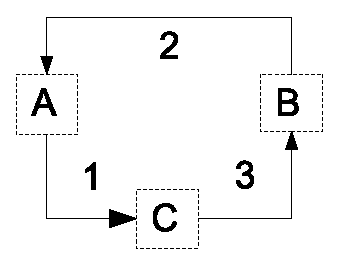
\includegraphics[width=0.5\textwidth]{img/ris_2_1}
\caption{Использование буферной переменной}
\label{ch02:refDrawing0}
\end{center}
\end{figure}

Если в операторе присваивания левая и правая часть это переменные разных типов, то \emph{происходит
преобразование}: значение переменной в правой части преобразуется к типу переменной в левой части. Следует учитывать,
что при этом можно потерять информацию или получить другое значение.

В \Sys{С++} существует возможность присваивания нескольким переменным одного и того же значения. Такая операция называется
\index{Операции!множественного присваивания}\emph{множественным присваиванием} и в общем виде может быть
записана так:

\Sys{имя\_1 = имя\_2 = … = имя\_N = значение;}

Запись \Sys{a=b=c=3.14159/6;}

означает, что переменным \Sys{a}, \Sys{b} и \Sys{c} было присвоено одно и то же
значение \Sys{3.14159/6}.

Операции +=, –=, *=, /= называют \index{Операции!составного присваивания}\emph{составным присваиванием}. В
таких операциях при вычислении выражения стоящего справа используется значение переменной из левой части, например так:

\Sys{x+=p; //Увеличение x на p, то же что и x=x+p.}

\Sys{x-=p; //Уменьшения x на p, то же что и x=x-p.}

\Sys{x*=p; //Умножение x на p, то же что и x=x*p.}

\Sys{x/=p; //Деление x на p, то же что и x=x/p.}

\subsection[Арифметические операции]{Арифметические операции}
Операции +, -, *, / относят к
\index{Операции!арифметические}\emph{арифметическим операциям}. Их назначение понятно и не требует
дополнительных пояснений. При программировании арифметических выражений следует придерживаться простых правил.
Соблюдать очерёдность выполнения арифметических операций. Сначала выполняются операции умножения и деления (1-й
уровень), а затем сложения и вычитания (2-й уровень). Операции одного уровня выполняются последовательно друг за
другом. Для изменения очерёдности выполнения операций используют скобки. Таблица \ref{ch02:refTable4} содержит примеры
записи алгебраических выражений.

\noindent
\begin{longtable}{|l|p{0.5\textwidth}|}
\caption{Примеры записи алгебраических выражений} \label{ch02:refTable4}\\
\hline
\Emph{Математическая запись}&\Emph{Запись на языке \Sys{С++}}\\
\hline \hline
\endfirsthead
\multicolumn{2}{c}%
{{\tablename\ \thetable{} --- продолжение}} \\
\hline
\Emph{Математическая запись}&\Emph{Запись на языке \Sys{С++}}\\
\hline \hline
\endhead
$\displaystyle 2\cdot a+b\cdot (c+d)$  & \Sys{2*a+b*(c+d)}\\\hline
$\displaystyle 3\cdot {\frac{a+b}{c+d}}$ & \Sys{3*(a+b)/(c+d)}\\\hline
$\displaystyle\frac{3\cdot a-2\cdot b}{c\cdot d}$ & \Sys{(3*a-2*b)/(c*d) или} \Sys{(3*a-2*b)/c/d}\\\hline
$\displaystyle\frac{(b-a)^2}{\displaystyle c+\displaystyle\frac{1}{d-2}}-\displaystyle\frac{a^2+1}{b^2+cd}$ & \Sys{(b-a)*(b-a)/(c+1/(d-2))-} \Sys{(a*a+1)/(b*b+c*d)}\\\hline
\end{longtable}

Операции \index{Операции!инкремента}\emph{инкремента} \Sys{++} и
\index{Операции!декремента}\emph{декремента} -{}-  так же причисляют к
арифметическим, так как они выполняют увеличение и уменьшение на единицу значения переменной. Эти операции имеют две
формы записи: префиксную (операция записывается перед операндом) и постфиксную (операция записывается после операнда).
Так, например оператор  \Sys{p=p+1;} можно представить в префиксной форме \Sys{++p;} и в
постфиксной \Sys{p++;}. Эти формы отличаются при использовании их в выражении. Если знак декремента
(инкремента) предшествует операнду, то сначала выполняется увеличение (уменьшение) значения операнда, а затем операнд
участвует в выражении. Например, 

%\noindent
\Sys{x=12;}

\Sys{y=++x; //В переменных x и y будет храниться значение 13. }

Если знак декремента (инкремента) следует после операнда, то сначала операнд участвует в выражении, а затем выполняется
увеличение (уменьшение) значения операнда:

%\noindent
\Sys{x=12;}

\Sys{y=x++; //Результат} --- \Sys{число 12 в переменной y, а в x} --- \Sys{13.}

Остановимся на \index{Операции!целочисленной арифметики}\emph{операциях целочисленной
арифметики}. 

Операция целочисленного деления \Sys{/} возвращает целую часть частного (дробная часть отбрасывается) в том
случае если она применяется к целочисленным операндам, в противном случае выполняется обычное деление: 11/4=2 или
11.0/4=2.75.

Операция остаток от деления \Sys{\%} применяется только к целочисленным операндам: 11\%4 = 3.

К \index{Операции!битовой арифметики}\emph{операциям битовой арифметики} относятся
следующие операции: \Sys{\&}, \Sys{{\textbar}}, \Sys{\^{}},
\Sys{\~{}}, \Sys{{\textless}{\textless}}, \Sys{{\textgreater}{\textgreater}}. В
операциях битовой арифметики действия происходят над двоичным представлением целых чисел. 

\emph{Арифметическое И} (\Sys{\&}). Оба операнда переводятся в двоичную систему, затем над
ними происходит логическое поразрядное умножение операндов по следующим правилам: 

1\&1=1, 1\&0=0, 0\&1=0, 0\&0=0. 

Например, если \Sys{А=14} и \Sys{В=24}, то их двоичное представление ---
\Sys{А=0000000000001110} и \Sys{В=0000000000011000}. В результате логического умножения
\Sys{A and B} получим \Sys{0000000000001000} или 8 в десятичной системе
счисления (рис. \ref{ch02:refDrawing1}). Таким образом, \Sys{A\&B=14\&24=8}.

\begin{figure}[htb]
\begin{center}
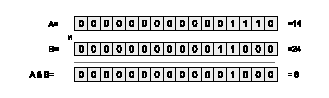
\includegraphics[width=0.5\textwidth]{img/ris_2_2}
\caption{Пример логического умножения}
\label{ch02:refDrawing1}
\end{center}
\end{figure}

\emph{Арифметическое ИЛИ} ({\textbar}). Здесь также оба операнда переводятся в двоичную
систему, после чего над ними происходит логическое поразрядное сложение операндов по следующим правилам:

\Sys{1{\textbar}1=1, 1{\textbar}0=1, 0{\textbar}1=1, 0{\textbar}0=0.} 

Например, результат логического сложения чисел \Sys{А=14} и \Sys{В=24} будет равен \Sys{A or B=30} 
(рис.~\ref{ch02:refDrawing2}). 

\begin{figure}[htb]
\begin{center}
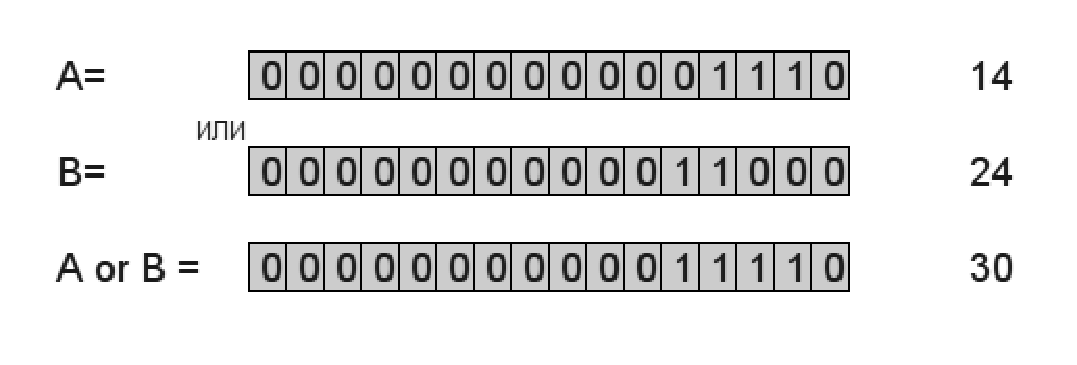
\includegraphics[width=0.5\textwidth]{img/ris_2_3}
\caption{Пример логического сложения}
\label{ch02:refDrawing2}
\end{center}
\end{figure}

\emph{Арифметическое исключающее ИЛИ} (\^{}). Оба операнда переводятся в двоичную
систему, после чего над ними происходит логическая поразрядная операция \^{} по следующим правилам:

\Sys{1\^{}1=0, 1\^{}0=1, 0\^{}1=1, 0\^{}0=0.}

\emph{Арифметическое отрицание} (\~{}). Эта операция выполняется над одним операндом.
Применение операции \~{} вызывает побитную инверсию двоичного представления числа 
(рис.~\ref{ch02:refDrawing3}).

\begin{figure}[htb]
\begin{center}
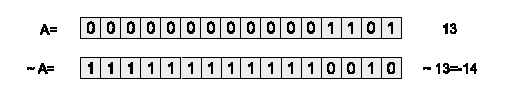
\includegraphics[width=0.5\textwidth]{img/ris_2_4}
\caption{Пример арифметического отрицания}
\label{ch02:refDrawing3}
\end{center}
\end{figure}

\emph{Сдвиг влево} (\Sys{M{\textless}{\textless}L}). Число
\Sys{M}, представленное в двоичной системе, сдвигается
влево на \Sys{L} позиций. Рассмотрим операцию \Sys{15 shl 3}. Число 15 в двоичной системе
имеет вид \Sys{1111}. При сдвиге его на 3 позиции влево получим \Sys{1111000}. В десятичной 
системе это двоичное число равно \Sys{120}.
Итак, \Sys{15 shl 3 =120} (рис.~\ref{ch02:refDrawing4}). Заметим, что сдвиг на один разряд влево соответствует
умножению на два, на два разряда --- умножению на четыре, на три --- умножению на восемь. Таким образом, операция
\Sys{M{\textless}{\textless}L} эквивалентна умножению числа \Sys{M} на 2 в степени \Sys{L}. 

\begin{figure}[htb]
\begin{center}
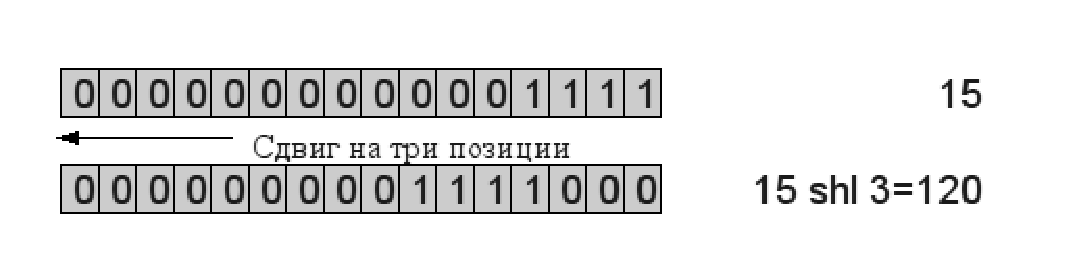
\includegraphics[width=0.5\textwidth]{img/ris_2_5}
\caption{Пример операции «Сдвиг влево»}
\label{ch02:refDrawing4}
\end{center}
\end{figure}

\emph{Сдвиг вправо} (\Sys{M{\textgreater}{\textgreater}L}). Число
\Sys{M}, представленное в двоичной системе, сдвигается вправо на 
\Sys{L} позиций, что эквивалентно целочисленному делению числа
\Sys{M} на 2 в степени \Sys{L}. Например, \Sys{15 shr 1=7} (рис.~\ref{ch02:refDrawing5}), \Sys{15 shr 3= 2}. 

\begin{figure}[htb]
\begin{center}
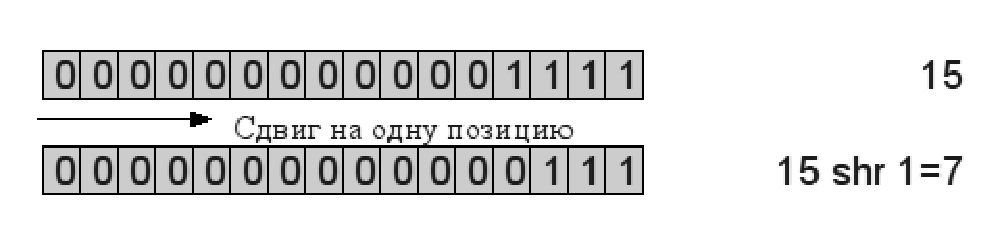
\includegraphics[width=0.5\textwidth]{img/ris_2_6}
\caption{Пример операции «Сдвиг вправо»}
\label{ch02:refDrawing5}
\end{center}
\end{figure}

\subsection[Логические операции]{Логические операции}
В \Sys{С++} определены следующие \index{Операции!логические}логические
операции {\textbar}{\textbar} (или), \Sys{\&\&} (и), \Sys{!} (не). Логические операции выполняются над логическими
значениями \Sys{true} (истина) и \Sys{false} (ложь). В языке \Sys{С++} ложь --- 0, истина --- любое
значение ${\neq}$ 0. В таблице~\ref{ch02:refTable5} приведены результаты логических операций.

\noindent
\begin{longtable}{|c|c|c|c|c|}
\caption{Логические операции} \label{ch02:refTable5}\\
\hline
\Emph{A}&\Emph{B}&\Emph{!A}&\Emph{A\&\&B}&\Emph{A{\textbar}{\textbar}B}\\
\hline \hline
\endfirsthead
\multicolumn{5}{c}%
{{\tablename\ \thetable{} --- продолжение}} \\
\hline
\Emph{A}&\Emph{B}&\Emph{!A}&\Emph{A\&\&B}&\Emph{A{\textbar}{\textbar}B}\\
\hline \hline
\endhead
0 & 0 & 1 & 0 & 0\\\hline
0 & 1 & 1 & 0 & 1\\\hline
1 & 0 & 0 & 0 & 1\\\hline
1 & 1 & 0 & 1 & 1\\\hline
\end{longtable}

\subsection[Операции отношения]{Операции отношения}
\index{Операции!отношения}\emph{Операции отношения} возвращают в качестве результата логическое значение.
Таких операций шесть:  \Sys{{\textgreater}}, \Sys{{\textgreater}=},
\Sys{{\textless}}, \Sys{{\textless}=}, \Sys{==}, \Sys{!=}.
Результат операции отношения --- логическое значение \Sys{true} (истина) или \Sys{false}
(ложь). 

\subsection[Условная операция]{Условная операция}
Для организации разветвлений в простейшем случае можно использовать \index{Операции!условная}\emph{условную
операцию} ? :. Эта операция имеет три операнда и в общем виде может быть представлена так:

\Sys{условие ? выражение1 : выражение2;}

Работает операция следующим образом. Если условие истинно (не равно 0), то результатом будет
\Sys{выражение1}, в противном случае \Sys{выражение2}. Например, операция
\Sys{y=x{\textless}0 ? -x : x;} записывает в переменную \Sys{y} модуль числа \Sys{х}.

\clearpage

\subsection[Операция преобразования типа]{Операция преобразования типа}

Для приведения выражения к другому типу данных в \Sys{С++} существует
\index{Операции!преобразования типа}\emph{операция преобразования типа}: 

\Sys{(тип) выражение;}

Например, в результате действий \Sys{x=5; y=x/2; z=(float) x/2;} переменная \Sys{y} примет
значение равное 2 (результат целочисленного деления), а переменная \Sys{z = 2.5}.

\subsection[Операция определения размера]{Операция определения размера}
Вычислить размер объекта или типа в байтах можно с помощью \emph{операции определения размера}, которая
имеет две формы записи:

\Sys{sizeof (тип);}\ \ \  или\ \ \ \Sys{sizeof выражение;}

Например, предположим, что была описана целочисленная переменная \Sys{int k=3;}. Исходя
из того, что тип \Sys{int} занимает в памяти 4 байта, в переменную
\Sys{m=sizeof k;} будет записано число 4.

В результате работы команд \Sys{double z=123.456; p=sizeof (k+z);} 
значение переменной \Sys{p} стало равно 8, т.~к. вещественный
тип \Sys{double} более длинный (8 байтов) по сравнению с типом
\Sys{int} (4 байта) и значение результата было преобразовано к более длинному типу. В
записи операции \Sys{sizeof (k+z)} были использованы скобки. Это
связано с тем, что операция определения типа имеет более высокий 
приоритет, чем операция сложения. При заданном
значении \Sys{z=123.456}; та же команда, но без скобок 
\Sys{p=sizeof k+z;} вычислит \Sys{p=4+123.456=127.456.}

Команда \Sys{s = sizeof "Hello"};
определит, что под заданную строку в памяти было выделено \Sys{s=6}
байтов, т. к. объект состоит из 5 символов и один байт на символ окончания строки.

\subsection[Операции с указателями]{Операции с указателями}
При работе с указателями часто используют операции \index{Операции!получение адреса}\emph{получения адреса}
\Sys{\&} и \index{Операции!разадресации}\emph{разадресации} \Sys{*} (табл.
\ref{ch02:refTable6}). 

\noindent
\begin{longtable}{|c|c|c|}
\caption{Операции получения адреса \Sys{\&} и
разадресации \Sys{*}} \label{ch02:refTable6}\\
\hline
\Emph{Описание}&\Emph{Адрес}&\Emph{Значение, хранящееся по адресу}\\
\hline \hline
\endfirsthead
\multicolumn{3}{c}%
{{\tablename\ \thetable{} --- продолжение}} \\
\hline
\Emph{Описание}&\Emph{Адрес}&\Emph{Значение, хранящееся по адресу}\\
\hline \hline
\endhead
\Sys{тип *p} & \Sys{p} & \Sys{*p}\\\hline
\Sys{тип p} & \Sys{\&p} & \Sys{p}\\\hline
\end{longtable}

\index{Указатель!получение адреса}\emph{Операция получения адреса} \Sys{\&} возвращает адрес
своего операнда. Например:

\Sys{float a; \ \ \ \ //Объявлена вещественная переменная а}

\Sys{float *adr\_a; //Объявлен указатель на тип float}

\Sys{adr\_a=\&a; \ \ \ //Оператор записывает в переменную adr\_a }

\Sys{\ \ \ \ \ \ \ \ \ \ \ \ \ //адрес переменной a }

\index{Указатель!разадресация}\emph{Операция разадресации} \Sys{*} возвращает значение
переменной, хранящееся по заданному адресу, т.е. выполняет действие, обратное операции \Sys{\&}:

\Sys{float a; \ \ \ \ //Объявлена вещественная переменная а.}

\Sys{float *adr\_a; \ \ //Объявлен указатель на тип float.}

\Sys{a=*adr\_a; \ \ \ \ //Оператор записывает в переменную a}

\Sys{\ \ \ \ \ //вещественное значение, хранящееся по адресу adr\_a.}


К указателям применяют \index{Операции!присваивания}\emph{операцию присваивания}. Это значит, что значение
одного указателя можно присвоить другому. Если указатели одного типа, то для этого применяют обычную операцию
\index{Указатель!присваивание}\emph{присваивания}: 

\Sys{//Описана вещественная переменная и два указателя.}

\Sys{float PI=3.14159,*p1,*p2;}

\Sys{//В указатели p1 и p2 записывается адрес переменной PI.}

\Sys{p1=p2=\&PI;}


Если указатели ссылаются на различные типы, то при присваивании значения одного указателя другому, необходимо
использовать преобразование типов. Без преобразования можно присваивать любому указателю указатель
\Sys{void*}. 

Рассмотрим пример работы с указателями различных типов:

\Sys{float PI=3.14159; \ \ //Объявлена вещественная переменная.}

\Sys{float *p1; \ \ \ \ //Объявлен указатель на float.}

\Sys{double *p2; \ \ \ //Объявлен указатель на double.}

\Sys{p1=\&PI; //Переменной p1 присваивается значение адреса PI.}

\Sys{p2=(double *)p1; \ \ //Указателю на double присваивается}

\Sys{\ \ \ \ \ \ \ \ \ \ \ \ //значение, которое ссылается на тип float.}

В указателях \Sys{p1} и \Sys{p2} хранится один и тот же адрес
(\Sys{p1=0012FF7C}), но значения, на которые они ссылаются разные (\Sys{*p1=3.14159},
\Sys{*p2=2.642140e-308}). Это связано с тем, указатель типа \Sys{*float} адресует 4 байта, а
указатель \Sys{*double} --- 8 байт. После присваивания \Sys{p2=(double *)p1;} при обращении к
\Sys{*p2} происходит следующее: к переменной, хранящейся по адресу \Sys{p1}, дописывается еще
следующих 4 байта из памяти. В результате значение \Sys{*p2} не совпадает со значением
\Sys{*p1}.

Таким образом, при преобразовании указателей разного типа приведение типов разрешает только синтаксическую проблему
присваивания. Следует помнить, что операция \Sys{*} над указателями различного типа, ссылающимися на один
и тот же адрес, возвращает различные значения.

Над адресами \Sys{С++} определены следующие
\index{Операции!арифметические}\emph{арифметические операции}:

\begin{itemize}
\item \index{Указатель!сложение с константой}\emph{сложение и вычитание указателей с
константой};
\item \index{Указатель!вычитание}\emph{вычитание одного указателя из другого};
\item \index{Указатель!инкремент}\emph{инкремент};
\item \index{Указатель!декремент}\emph{декремент}.
\end{itemize}

\emph{Сложение и вычитание указателей с константой} \Sys{n} означает, что указатель
перемещается по ячейкам памяти на столько байт, сколько занимает \Sys{n} переменных того типа на который
он указывает. Например, пусть указатель имеет символьный тип и его значение равно 100. Результат сложения этого
указателя с единицей --- 101, так как для хранения переменной типа \Sys{char} требуется один байт. Если же
значение указателя равно 100, но он имеет целочисленный тип, то результат его сложения с единицей будет составлять 104,
так как для переменной типа \Sys{int} отводится четыре байта.

Эти операции применимы только к указателям одного типа и имеют смысл в основном при работе со структурными типами
данных, например массивами.

Фактически получается, что значение указателя изменяется на величину \Sys{sizeof(тип)}. Если указатель на
определенный тип увеличивается или уменьшается на константу, то его значение изменяется на величину этой константы,
умноженную на размер объекта данного типа. Например:

\Sys{//Объявление массива из 10 элементов.}

\Sys{double mas[10]=\{1.29,3.23,7.98,5.54,8.32,2.48,7.1\}; }

\Sys{double *p1; \ \ //Объявление указателя на double}

\Sys{p1=\&mas[0]; \ \ //Присвоение указателю адреса}

\Sys{\ \ \ \ \ \ \ \ //нулевого элемента массива.}

\Sys{p1=p1+3;\ \ \ \ //Увеличение значения адреса на 3*8=24}

\Sys{\ \ \ \ \ \ \ \ //(размер типа double), в результате указатель}

\Sys{\ \ \ \ \ \ //сместится на три ячейки, размером double каждая.}


\emph{Вычитание двух указателей} определяет сколько переменных данного типа размещается между указанными
ячейками. Разность двух указателей это разность их значений, деленная на размер типа в байтах. Так разность указателей
на третий и нулевой элементы массива равна трем, а на третий и девятый --- шести. Суммирование двух указателей не
допускается.

Операции \emph{инкремента} и \emph{декремента}, соответственно, увеличивают или уменьшают
значение адреса:

\Sys{double *p1;}

\Sys{float *p2; }

\Sys{int *i; }

\Sys{p1++; \ \ //Увеличение значения адреса на 8.}

\Sys{p2++; \ \ //Увеличение значения адреса на 4.}

\Sys{i++; \ \ \ \ //Увеличение значения адреса на 4.}

К указателям так же применимы {операции отношения} \Sys{==}, \Sys{!=},
\Sys{{\textless}}, \Sys{{\textgreater}}, \Sys{{\textless}=},
\Sys{{\textgreater}=}. Иными словами указатели можно сравнивать. Например, если \Sys{i}
указывает на пятый элемент массива, а \Sys{j} на первый, то отношение \Sys{i{\textgreater}j}
истинно. Кроме того, любой указатель всегда можно сравнить на равенство с константой нулевого указателя
(NULL)\footnote{Константу нулевого указателя можно присвоить любому указателю и такой указатель при сравнении не будет
равен любому реальному указателю.}. Однако, все эти утверждения верны, если речь идёт об указателях ссылающихся на один
массив. В противном случае результат арифметических операций и операций отношения будет не определён.

\section[Стандартные функции]{Стандартные функции}\label{ch02:7}
В C++ определены \index{Функции!стандартные}\emph{стандартные}\index{Функции}
\emph{функции} над арифметическими операндами\footnote{Работа с математическими функциями
возможно только при подключении директивы {math.h} (п.~\ref{ch02:6})}. В таблице \ref{ch02:refTable7} приведены
некоторые из них.

\noindent
\begin{longtable}{|l|p{0.7\textwidth}|}
\caption{Стандартные математические функции} \label{ch02:refTable7}\\
\hline
\Emph{Обозначение}&\Emph{Действие}\\
\hline \hline
\endfirsthead
\multicolumn{2}{c}%
{{\tablename\ \thetable{} --- продолжение}} \\
\hline
\Emph{Обозначение}&\Emph{Действие}\\
\hline \hline
\endhead
\Sys{abs(x)} & Модуль целого числа $x$\\\hline
\Sys{fabs(x)} & Модуль вещественного числа $x$\\\hline
\Sys{sin(x)} & Синус числа $x$\\\hline
\Sys{cos(x)} & Косинус числа $x$\\\hline
\Sys{tan(x)} & Тангенс числа $x$\\\hline
\Sys{atan(x)} & Арктангенс числа $x$,  $x\in (-{\frac{i\pi}{2}};\frac{i\pi}{2})$\\\hline
\Sys{acos(x)} & Арккосинус числа $x$\\\hline
\Sys{asin(x)} & Арксинус числа $x$\\\hline
\Sys{exp(x)} & Экспонента, $e^x$\\\hline
\Sys{log(x)} & Натуральный логарифм, ($x>0$)\\\hline
\Sys{log10(x)} & Десятичный логарифм, ($x>0$) \\\hline
\Sys{sqrt(x)} & Корень квадратный, ($x>0$)\\\hline
\Sys{pow(x,y)} & Возведение числа $x$ в степень $y$\\\hline
\Sys{ceil(x)} & Округление числа $x$ до ближайшего большего целого\\\hline
\Sys{floor(x)} & Округление числа $x$ до ближайшего меньшего целого\\\hline
\end{longtable}

Примеры записи математических выражений с использованием встроенных функций представлены в таблице \ref{ch02:refTable8}.

\noindent
\begin{longtable}{|p{0.4\textwidth}|p{0.5\textwidth}|}
\caption{Примеры записи математических выражений} \label{ch02:refTable8}\\
\hline
\Emph{Математическая запись}&\Emph{Запись на языке \Sys{С++}}\\
\hline \hline
\endfirsthead
\multicolumn{2}{c}%
{{\tablename\ \thetable{} --- продолжение}} \\
\hline
\Emph{Математическая запись}&\Emph{Запись на языке \Sys{С++}}\\
\hline \hline
\endhead
$
\sqrt[{3}]{(a+b)^{2}}
$
 &
\Sys{pow((a+b)*(a+b),1./3)} или

\Sys{pow(pow(a+b,2),1./3)}\\\hline
$
\cos ^{4}(x)
$
 &
\Sys{pow(cos(x), 4)}\\\hline
$
e^{2x}
$
 &
\Sys{exp(2*x)}\\\hline
$
e^{5\sin (\frac{x}{2})}
$
 &
\Sys{exp(5*sin(x/2))}\\\hline
$
\sin ^{2}(\sqrt{x})
$
 &
\Sys{pow(sin(sqrt(x)),2)}\\\hline
$
\ln (|x-2|)
$
 &
\Sys{log(fabs(x-2))}\\\hline
$
\log _{b}a
$
 &
\Sys{log(a)/log(b)}\\\hline
$
\displaystyle\frac{lg(x^{2}+1)}{lg(4)}
$
 &
\Sys{log10(x*x+1)/log10(4)}\\\hline
$
\sin (x^{2}+y^{2})+\cos \frac{(x^{2}+y^{2})}{2\cdot y}+$

$+\sqrt{x^{2}+y^{2}}
$
 &
\Sys{z=x*x+y*y;}

\Sys{sin(z)+cos(z/(2*y))+sqrt(z);}\\\hline
\end{longtable}

Определенную проблему представляет применение функции \Sys{pow(x,y)}. При программировании выражений,
содержащих возведение в степень, надо внимательно проанализировать значения, которые могут принимать
$x$ и $y$, так как в некоторых случаях возведение
$x$ в степень $y$ невыполнимо.

Так, ошибка возникает, если $x$ --- отрицательное число, а $y$ --- дробь. Предположим,
что $y$ --- правильная дробь вида  $\frac{k}{m}$. Если знаменатель $m$ четный, это
означает вычисление корня четной степени из отрицательного числа, а значит, операция не 
может быть выполнена. В
противном случае, если знаменатель $m$ нечетный, можно воспользоваться выражением 
\Sys{z = –pow(fabs(x),y)}. Например, вычисление кубического корня из вещественного числа 
можно представить командой:

\noindent\Sys{z=(x{\textless}0) ? -pow(fabs(x),(double) 1/3) : pow(x,(double) 1/3);}

\section[Структура программы]{Структура программы}\label{ch02:8}
\index{Программа}\emph{Программа} на языке \Sys{С++} \index{Программа!структура}состоит из
\emph{функций}, \emph{описаний} и \emph{директив процессора}. 

Одна из функций должна обязательно носить имя \Sys{main}. Элементарное описание функции имеет вид:

\begin{lstlisting}
`\Sys{тип\_результата имя\_функции (параметры)}`
{
    `\Sys{оператор1;}`
    `\Sys{оператор2;}`
    `\Sys{…}`
    `\Sys{операторN;}`
}
\end{lstlisting}

Здесь, \Sys{тип\_результата} --- это тип того значения, которое функция должна вычислить (если функция не
должна возвращать значение, указывается тип \Sys{void}), \Sys{имя\_функции} --- имя, с которым
можно обращаться к этой функции, \Sys{параметры} --- список аргументов функции (может отсутствовать),
\Sys{оператор1}, \Sys{оператор2},\Sys{…}, \Sys{операторN} --- операторы, представляющие
тело функции, они обязательно заключаются в фигурные скобки и каждый оператор заканчивается точкой с запятой. Как
правило программа на \Sys{С++} состоит из одной или нескольких, не вложенных друг в друга функций.

Основному тексту программы предшествуют \index{Директивы}\emph{директивы препроцессора}
предназначенные для \emph{подключения библиотек}, которые в общем виде
выглядят так:

\Sys{\#include {\textless}имя\_файла{\textgreater}}

Каждая такая строка дает компилятору команду присоединить программный код, который хранится в отдельном файле с
расширением \Sys{.h}. Такие файлы называют \emph{файлами заголовков}. С их помощью можно
выполнять ввод-вывод данных, работать с математическими функциями, преобразовывать данные, распределять память и многое
другое. Например, описание стандартных математических функций находится в заголовочном файле \Sys{math.h}.

Общую структуру программы на языке \Sys{С++} можно записать следующим образом:
\begin{lstlisting}
`\Sys{директивы процессора}`
`\Sys{описание глобальных переменных}`
`\Sys{тип\_результата main(параметры)}`
{
`\Sys{описание переменных главной функции;}`
  `\Sys{операторы главной функции;}`
}

`\Sys{тип\_результата имя1(параметры1)}`
{
`\Sys{описание переменных функции имя1;}`
  `\Sys{операторы1;}`
}

`\Sys{тип\_результата имя2(параметры2)}`
{
`\Sys{описание переменных функции имя2;}`
  `\Sys{операторы2;}`
}

................................

`\Sys{тип\_результата имяN(параметрыN)}`
{
`\Sys{описание переменных функции имяN;}`
  `\Sys{операторыN;}`
}
\end{lstlisting}

По месту объявления переменные в языке Си можно разделить на три класса: локальные, глобальные и формальные параметры
функции.

\index{Переменная!локальная}\emph{Локальные переменные} объявляются внутри функции и доступны только в ней.
Например:
\begin{lstlisting}
int main()
{
//`В функции main определена вещественная переменная` s,
    float s; 
    s=4.5;   //`и ей присвоено значение `4.5.
}
int f1()
{
//`В функции` f1 `описана другая переменная` s,
    int s; 
    s=6;   //`ей присвоено значение` 6.
}
int f2()
{
//`В функции `f2 `определена еще одна переменная` s,
	long int s; 
	s=25;      //`ей присвоено значение` 25.
}
\end{lstlisting}

\index{Переменная!глобальная}\emph{Глобальные переменные} описываются до всех функций и доступны из любого
места программы. Например:
\begin{lstlisting}
float s; //`Определена глобальная переменная` s.
int main()
{
//`В главной функции переменной` s `присваивается значение` 4.5.
	s=4.5; 
}
int f1()
{
//`В функции` f1 `переменной `s `присваивается значение` 6.
	s=6;
}
int f2()
{
//`В функции `f2 `переменной` s `присваивается значение` 2.1.
    s=2.1;
\end{lstlisting}

Формальные параметры функций описываются в списке параметров функции. Работа с функциями подробно описана в главе~\ref{ch04}.

\section[Ввод и вывод данных]{Ввод и вывод данных}\label{ch02:9}
{Ввод-вывод данных} в языке \Sys{С++} осуществляется либо с помощью функций ввода-вывода в стиле \Sys{С}, либо с
использованием библиотеки классов \Sys{С++}. Преимущество объектов \Sys{С++} в том, что они легче 
в использовании, особенно если
ввод-вывод достаточно простой. Функции ввода-вывода унаследованные от \Sys{С} более громоздкие, 
но более гибко управляют
форматированным выводом данных.

Функция

\Sys{printf(строка форматов, список выводимых переменных);}

выполняет форматированный \index{Функции!вывод данных}\emph{вывод переменных}, указанных в списке, в
соответствии со строкой форматов. 

Функция

\Sys{scanf(строка форматов, список адресов вводимых переменных);}

выполняет \index{Функции!ввод данных}\emph{ввод переменных}, адреса которых указанны в списке, в
соответствии со строкой форматов. 

\emph{Строка форматов} содержит символы, которые будут выводиться на экран или запрашиваться с клавиатуры и
так называемые спецификации. \emph{Спецификации} это строки, которые начинаются символом
\Sys{\%} и выполняют управление форматированием:

\Sys{\% флаг ширина . точность модификатор тип}

Параметры \Sys{флаг}, \Sys{ширина}, \Sys{точность} и
\Sys{модификатор} в спецификациях могут отсутствовать. Значения параметров спецификаций приведены в
таблице \ref{ch02:refTable9}.


\noindent
\begin{longtable}{|l|p{0.7\textwidth}|}
\caption{Символы управления} \label{ch02:refTable9}\\
\hline
\Emph{Параметр}&\Emph{Назначение}\\
\hline \hline
\endfirsthead
\multicolumn{2}{c}%
{{\tablename\ \thetable{} --- продолжение}} \\
\hline
\Emph{Параметр}&\Emph{Назначение}\\
\hline \hline
\endhead
\multicolumn{2}{|c|}{Флаги}\\\hline
\Sys{{}-} &
Выравнивание числа влево. Правая сторона дополняется пробелами. По умолчанию выравнивание вправо.\\\hline
\Sys{+} &
Перед числом выводится знак «\Sys{+}» или «\Sys{{}-}»\\\hline
\Sys{Пробел} &
Перед положительным числом выводится пробел, перед отрицательным «\Sys{–}»\\\hline
\Sys{\#} &
Выводится код системы счисления: \Sys{0} --- перед восьмеричным числом, \Sys{0х}
(\Sys{0Х}) перед шестнадцатеричным числом.\\\hline
\multicolumn{2}{|c|}{Ширина}\\\hline
\Sys{n} &
Ширина поля вывода. Если \Sys{n} позиций недостаточно, то поле вывода расширяется до минимально
необходимого. Незаполненные позиции заполняются пробелами.\\\hline
\Sys{0n} &
То же, что и \Sys{n}, но незаполненные позиции заполняются нулями.\\\hline
\multicolumn{2}{|c|}{Точность}\\\hline
\centering \Sys{ничего} &
Точность по умолчанию\\\hline
\Sys{n} &
Для типов \Sys{e}, \Sys{E}, \Sys{f }выводить \Sys{n} знаков после
десятичной точки\\\hline
\multicolumn{2}{|c|}{Модификатор}\\\hline
\Sys{h} &
Для \Sys{d}, \Sys{i}, \Sys{o}, \Sys{u}, \Sys{x},
\Sys{X} тип \Sys{short int}.\\\hline
\Sys{l} &
Для \Sys{d}, \Sys{i}, \Sys{o}, \Sys{u}, \Sys{x},
\Sys{X} тип \Sys{long int}.\\\hline
\multicolumn{2}{|c|}{Тип}\\\hline
\Sys{с} &
При вводе символьный тип \Sys{char}, при выводе один байт.\\\hline
\Sys{d} &
Десятичное \Sys{int} со знаком.\\\hline
\Sys{i} &
Десятичное \Sys{int} со знаком.\\\hline
\Sys{o} &
Восьмеричное \Sys{int} \Sys{unsigned}.\\\hline
\Sys{u} &
Десятичное \Sys{int unsigned}.\\\hline
\Sys{x, X} &
Шестнадцатеричное \Sys{int unsigned}, при \Sys{х} используются символы
\Sys{a}{}-\Sys{f}, при \Sys{Х} --- \Sys{A }{}-
\Sys{F}.\\\hline
\Sys{f} &
Значение со знаком вида \Sys{[-]dddd.dddd}.\\\hline
\Sys{e} &
Значение со знаком вида \Sys{[-]d.dddde[+{\textbar}-]ddd}.\\\hline
\Sys{E} &
Значение со знаком вида \Sys{[-]d.ddddE[+{\textbar}-]ddd}.\\\hline
\Sys{g} &
Значение со знаком типа \Sys{e} или \Sys{f }в зависимости от значения и точности.\\\hline
\Sys{G} &
Значение со знаком типа \Sys{e} или \Sys{F} в зависимости от значения и точности.\\\hline
\Sys{s} &
Строка символов.\\\hline
\end{longtable}

Кроме того, строка форматов может содержать некоторые специальные символы, которые приведены в таблице
\ref{ch02:refTable10}.
\noindent
\begin{longtable}{|l|p{0.7\textwidth}|}
\caption{Специальные символы} \label{ch02:refTable10}\\
\hline
\Emph{Символ}&\Emph{Назначение}\\
\hline \hline
\endfirsthead
\multicolumn{2}{c}%
{{\tablename\ \thetable{} --- продолжение}} \\
\hline
\Emph{Символ}&\Emph{Назначение}\\
\hline \hline
\endhead
\Sys{{\textbackslash}b} &
Сдвиг текущей позиции влево.\\\hline
\Sys{{\textbackslash}n} &
Перевод строки.\\\hline
\Sys{{\textbackslash}r} &
Перевод в начало строки, не переходя на новую строку.\\\hline
\Sys{{\textbackslash}t} &
Горизонтальная табуляция.\\\hline
\Sys{{\textbackslash}’} &
Символ одинарной кавычки.\\\hline
\Sys{{\textbackslash}’’} &
Символ двойной кавычки.\\\hline
\Sys{{\textbackslash}?} &
Символ \Sys{?}\\\hline
\end{longtable}

Первой строкой программы, в которой будут применяться функции ввода-вывода языка С, должна быть директива
\Sys{\#include {\textless}stdio.h{\textgreater}}. Заголовочный файл \Sys{stdio.h} содержит
описание функций ввода-вывода. 

Рассмотрим работу функций на примере следующей задачи.

\prg{Зная \Sys{a}, \Sys{b},
\Sys{c} --- длины сторон треугольника, вычислить площадь \Sys{S} и периметр
\Sys{P} этого треугольника.}{gl02:prg2} 

Входные данные: \Sys{a}, \Sys{b}, \Sys{c.} Выходные данные:
\Sys{S}, \Sys{P}. 

Для вычисления площади применим формулу Герона:

$S=\sqrt{r\cdot (r-a)\cdot (r-b)\cdot (r-c)}$, где $r=\frac{a+b+c}{2}$ --- полупериметр.

Далее приведены две программы для решения данной задачи и результаты их работы 
(рис.~\ref{ch02:refDrawing6}--\ref{ch02:refDrawing7}).
Сравните работу функций \Sys{printf} и \Sys{scanf} в этих программах.
\begin{lstlisting}
//`ЗАДАЧА~\ref{gl02:prg2} Вариант первый`
#include <iostream>
#include <stdio.h>
#include <math.h>
using namespace std;
int main()
{
  float a,b,c,S,r;  //`Описание переменных.`
  printf("a=");	    //`Вывод на экран символов` a=.
  //`В функции scanf для вычисления адреса`
  //`переменной применяется операция` &.
  scanf("%f",&a);   //`Запись в переменную а значения`
                    //`введенного с клавиатуры`.
  printf("b=");     //`Вывод на экран символов` b=.
  scanf("%f",&b);   //`Запись в переменную` b `значения`
                    //`введенного с клавиатуры.`
  printf("c=");     //`Вывод на экран символов` c=
  scanf("%f",&c);   //`Запись в переменную c значения`
                    //`введенного с клавиатуры.`
  r=(a+b+c)/2;      //`Вычисление полупериметра.`
  S=sqrt(r*(r-a)*(r-b)*(r-c)); //`Вычисление площади треугольника.`
  printf("S=%5.2f \t",S); //`Вывод символов` S=, 
                          //`значения` S `и символа`
                          //`табуляции` \t.
                          //`Спецификация` %5.2f
                          //`означает, что будет` 
                          //`выведено вещественное` 
                          //`число из пяти знаков`,
                          //`два из которых после точки.`
  printf("p=%5.2f \n",2*r); //`Вывод символов` p=,
                          //`значения выражения` 2*r
                          //`и символа окончания строки.`
  //`Оператор` printf("S=%5.2f \t p=%5.2f \n",S,2*r);
  //`выдаст тот же результат.`
  return 0;
}
\end{lstlisting}

\begin{figure}[htb]
\begin{center}
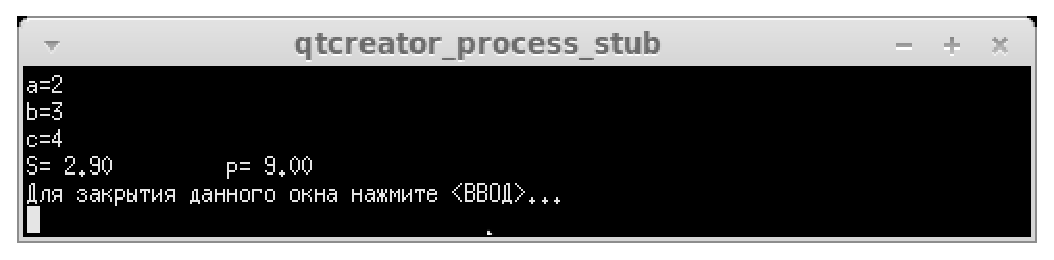
\includegraphics[width=0.8\textwidth]{img/ris_2_7}
\caption{Результаты работы программы к задаче \ref{gl02:prg2} (вариант 1)}
\label{ch02:refDrawing6}
\end{center}
\end{figure}

\begin{lstlisting}
//`ЗАДАЧА~\ref{gl02:prg2}. Вариант второй`
#include <iostream>
#include <stdio.h>
#include <math.h>
using namespace std;
int main()
{
  float a,b,c,S,r;
  printf("Vvedite a, b, c \n");  //`Вывод на экран строки символов.`
  scanf("%f%f%f",&a,&b,&c); //`Ввод значений.`
  r=(a+b+c)/2;
  S=sqrt(r*(r-a)*(r-b)*(r-c));
  printf("S=%5.2f \t p=%5.2f \n",S,2*r); //`Вывод результатов.`
  return 0;
}
\end{lstlisting}

\begin{figure}[htb]
\begin{center}
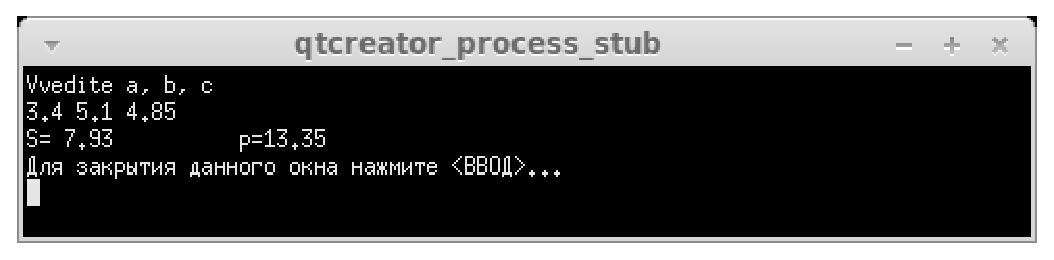
\includegraphics[width=0.8\textwidth]{img/ris_2_8}
\caption{Результаты работы программы к задаче \ref{gl02:prg2} (вариант 2)}
\label{ch02:refDrawing7}
\end{center}
\end{figure}

\subsection[Объектно-ориентированные средства ввода-вывода.]{Объектно-ориентированные средства ввода-вывода.}
Описание объектов для управления вводом-выводом содержится в заголовочном файле \Sys{iostream}. При
подключении этого файла с помощью директивы \Sys{\#include {\textless}iostream{\textgreater}} в программе
автоматически создаются \emph{объекты-потоки}\footnote{Поток --- виртуальный канал связи, создаваемый в
программе для передачи данных} \Sys{cin} для \emph{ввода с клавиатуры} и
\Sys{cout} для \emph{вывода на экран}, а так же операции помещения в поток
\Sys{{\textless}{\textless}} и чтения из потока \Sys{{\textgreater}{\textgreater}}.

Итак, с помощью объекта \Sys{cin} и операции \Sys{{\textgreater}{\textgreater}} можно ввести
значение любой переменной. Например, если переменная \Sys{i} описана как целочисленная, то команда
\Sys{cin{\textgreater}{\textgreater} i; }означает, что в переменную \Sys{i} будет записано
некое целое число, введенное с клавиатуры. Если нужно ввести несколько переменных, следует написать
\Sys{cin{\textgreater}{\textgreater}x{\textgreater}{\textgreater}y{\textgreater}{\textgreater}z;}.

Объект \Sys{cout} и операция \Sys{{\textless}{\textless}} позволяют вывести на экран значение
любой переменной или текст. Текст необходимо заключать в двойные кавычки, кроме того, допустимо применение специальных
символов \Sys{{\textbackslash}t} и \Sys{{\textbackslash}n} (таблица~\ref{ch02:refTable10}).
Запись c\Sys{out{\textless}{\textless}i;} означает вывод на экран значения переменной
\Sys{i}. А команда
\Sys{cout{\textless}{\textless}x{\textless}{\textless}"{\textbackslash}t"{\textless}{\textless}y;} выведет
на экран значения переменных \Sys{x} и \Sys{y} разделенные символом табуляции.

\prg{Дано трехзначное число. Записать его цифры в обратном порядке и вывести на
экран новое число.}{gl2:prg3}

Разберем решение данной задачи на конкретном примере. Здесь будут использоваться операции целочисленной арифметики. 

Пусть \Sys{P=456}. Вычисление остатка от деления числа \Sys{P} на \Sys{10} даст
его последнюю цифру (количество единиц в числе \Sys{P}):
\Sys{456 \% 10 =6.}

Операция деления нацело числа \Sys{P} на \Sys{10} позволит уменьшить количество разрядов и
число станет двузначным:

\Sys{456 / 10 = 45.}

Остаток от деления полученного числа на \Sys{10} будет следующей цифрой числа \Sys{P}
(количество десятков в числе \Sys{P}):

\Sys{45 \% 10 = 5.}

Последнюю цифру числа \Sys{P} (количество сотен) можно найти так:

\Sys{456 / 100 = 4.}

Так как в задаче требовалось записать цифры числа \Sys{P} в обратном порядке, значит в новом числе будет
\Sys{6} сотен, \Sys{5} десятков и \Sys{4} единицы:

\Sys{S = 6*100 + 5*10 + 4 = 654.}

Далее приведен текст программы, реализующей данную задачу для любого трехзначного числа.

\begin{lstlisting}
#include <iostream>
using namespace std;
int main(int argc, char *argv[])
{
unsigned int P, S;  //`Определение целочисленных`
                    //`переменных без знака`.
cout<<"P=";         //`Вывод на экран символов` P=.
cin>>P;             //`Ввод заданного числа` P.
S=P%10*100+P/10%10*10+P/100;  //`Вычисление нового числа` S.
cout<<"S="<<S<<endl;          //`Вывод на экран символов` S=
                              //`и значения переменной` S.
return 0;
}
\end{lstlisting}

\prg{Пусть целочисленная переменная \Sys{i} и вещественная переменная
\Sys{d} вводятся с клавиатуры. Определить размер памяти, отведенной для хранения этих переменных и их
суммы, в байтах. Вычислить сколько памяти будет выделено для хранения строки \Sys{С Новым Годом!}. Вывести
на экран размеры различных типов данных языка \Sys{С++} в байтах.}{gl02:prg4} 

Далее приведён текст программы.
\begin{lstlisting}
#include <iostream>
using namespace std;
int main()
{
int i;     //`Определение целочисленной переменной`.
double d;  //`Определение вещественной переменной`.

cout<<"i= "; cin>>i;  //`Ввод переменной` i.
cout<<"d= "; cin>>d;  //`Ввод переменной` d.
//`Размер памяти`, `отведенной под переменную` i.
cout<<"`Размер` i: "<<sizeof i<<"\n";
//`Размер памяти, отведенной под переменную` d.
cout<<"`Размер` d: "<<sizeof d<<"\n";
//`Размер памяти, отведенной под значение выражения` i+d.
cout<<"`Размер` i+d: "<<sizeof (i+d)<<"\n";
cout<<"`Размер строки <С Новым Годом!>:`";
//`Размер памяти, отведенной под строку.`
cout<<sizeof "`С Новым годом!`"<<"\n";
//`Вычисление размеров различных типов данных:`
cout<<"`Размер` char: "<<sizeof (char)<<"\n";
cout<<"`Размер` int: "<<sizeof (int)<<"\n";
cout<<"`Размер` short int: "<<sizeof (short int)<<"\n";
cout<<"`Размер` long int: "<<sizeof (long int)<<"\n";
cout<<"`Размер` long long int:";
cout<<sizeof (long long int)<<"\n";
cout<<"`Размер` float: "<<sizeof (float)<<"\n";
cout<<"`Размер` double: "<<sizeof (double)<<"\n";
cout<<"`Размер` long double: "<<sizeof (long double)<<"\n";
return 0;
}
\end{lstlisting}

Результаты работы программы\footnote{Обратите внимание, что при использовании кодировки utf-16 один кириллический символ
занимает в памяти занимает 2 байта.}

\begin{verbatim}
i= 23 
d= 45.76 
Размер i: 4 
Размер d: 8 
Размер i+d: 8 
Размер <С Новым годом!>:26 
Размер char: 1 
Размер int: 4 
Размер short int: 2 
Размер long int: 4 
Размер long long int:8 
Размер float: 4 
Размер double: 8 
Размер long double: 12 
\end{verbatim}

\section[Задачи для самостоятельного решения]{Задачи для самостоятельного решения}
\subsection[Ввод-вывод данных. Операция присваивания.]{Ввод-вывод данных. Операция присваивания.}
Разработать программу на языке \Sys{С++}. Все входные и выходные данные в задачах --- \emph{вещественные числа}.
Для ввода и вывода данных использовать функции \Sys{scanf} и \Sys{printf}.
\begin{enumerate}
\item Даны катеты прямоугольного треугольника $a$ и $b$. Найти гипотенузу
$c$ и углы треугольника ${\alpha}$, ${\beta}$, ${\chi}$.

\item Известна гипотенуза $c$ и прилежащий угол ${\alpha}$ прямоугольного
треугольника. Найти площадь треугольника $S$ и угол~${\beta}$.

\item Известна диагональ квадрата $d$. Вычислить площадь $S$ и периметр
$P$ квадрата.

\item Дан диаметр окружности $d$. Найти ее длину $L$ и площадь круга~$S$.

\item Даны три числа --- $a$, $b$, $c$. Найти их среднее
арифметическое и среднее геометрическое.

\item Даны катеты прямоугольного треугольника $a$ и $b$. Найти его гипотенузу
$c$ и периметр~$P$.

\item Дан длина окружности $L$. Найти ее радиус $R$ и площадь круга~$S$.

\item Даны два ненулевых числа $a$ и $b$. Найти сумму $S$,
разность $R$, произведение $P$ и частное $d$ их квадратов.

\item Поменять местами содержимое переменных $A$ и $B$ и вывести новые значения $A$ и~$B$.

\item Точки $A$ и $B$ заданы координатами на плоскости:
$A(x_1,y_1)$, $B(x_2,y_2)$. Найти длину отрезка $AB$.

\item Заданы два катета прямоугольного треугольника $a$ и $b$. Вычислить его
площадь $S$ и периметр $P$.

\item Даны переменные $A$, $B$, $C$. Изменить их значения,
переместив содержимое $A$ в $B$, $B$ --- в $C$,
$C$ --- в $A$, и вывести новые значения переменных $A$,
$B$, $C$.

\item Известна диагональ ромба $d$. Вычислить его площадь $S$ и периметр
$P$.

\item Найти значение функции  $y=4\cdot (x+1)^{3}+5\cdot (x-1)^{5}+2$ и ее производной при заданном значении
$x$.

\item Даны два ненулевых числа $a$ и $b$. Найти сумму $S$,
разность $R$, произведение $P$ и частное $D$ их модулей.

\item Известны координаты вершин квадрата $ABCD$:
$A(x_1,y_1)$ и $C(x_2,y_2)$. Найти его площадь $S$ и периметр~$P$.

\item Даны длины сторон прямоугольника $a$ и $b$. Найти его площадь
$S$ и периметр~$P$.

\item Известно значение периметра $P$ равностороннего треугольника. Вычислить его площадь~$S$.

\item Задан периметр квадрата $P$. Вычислить сторону квадрата $a$, диагональ
$d$ и площадь~$S$.

\item Дана сторона квадрата $a$. Вычислить периметр квадрата $P$, его площадь
$S$ и длину диагонали~$d$.

\item Три точки заданы координатами на плоскости:
$A(x_1,y_1)$, $B(x_2,y_2)$ и $C(x_3,y_3)$. Найти длины
отрезков $AB$ и $BC$.

\item Даны переменные A, B, C. Изменить их значения, переместив содержимое $A$ в
$C$, $C$ --- в $B$, $B$ --- в
$A$, и вывести новые значения переменных $A$, $B$,
$C$.

\item Даны числа --- $a_1$, $a_2$, $a_3$, $a_4$, $a_5$.
Найти их среднее арифметическое и среднее геометрическое значения.

\item Найти значение функции  $y=\frac{3}{2}\cdot (x+3)^{4}-\frac{1}{5}\cdot (x-1)^{5}$  и ее производной при заданном
значении $x$.

\item Точки $A$ и $B$ заданы координатами в пространстве:
$A(x_1, y_1, z_1)$, $B(x_2, y_2, z_2)$. Найти длину отрезка $AB$.
\end{enumerate}

\subsection[Операции целочисленной арифметики.]{Операции целочисленной арифметики.}
Разработать программу на языке \Sys{С++}. Все входные данные в задачах --- {целые числа}. Для ввода и вывода
данных использовать объектно-ориентированные средства ввода-вывода.

\begin{enumerate}
\item Расстояние $L$ задано в сантиметрах. Найти количество полных метров в нем и остаток в
сантиметрах.
\item Масса $M$ задана в килограммах. Найти количество полных тонн в ней и остаток в килограммах.
\item Дан размер файла $B$в байтах. Найти количество полных килобайтов, которые занимает данный файл
и остаток в байтах.
\item Дано двузначное число. Вывести на экран количество десятков и единиц в нем.
\item Дано двузначное число. Найти сумму его цифр.
\item Дано двузначное число. Найти произведение его цифр.
\item Дано двузначное число. Вывести число, полученное при перестановке цифр исходного числа.
\item Дано трехзначное число. Определить сколько в нем единиц, десятков и сотен.
\item Дано трехзначное число. Найти сумму его цифр.
\item Дано трехзначное число. Найти произведение его цифр.
\item Дано трехзначное число. Вывести число, полученное при перестановке цифр сотен и десятков исходного числа.
\item Дано трехзначное число. Вывести число, полученное при перестановке цифр сотен и единиц исходного числа.
\item Дано трехзначное число. Вывести число, полученное при перестановке цифр десятков и единиц исходного числа.
\item С начала суток прошло N секунд. Найти количество полных минут, прошедших с начала суток и остаток в секндах.
\item С начала суток прошло N секунд. Найти количество полных часов, прошедших с начала суток и остаток в секндах.
\item Дано двузначное число $\alpha\le 88$. Вывести на экран число, которое получится если каждую цифру числа
$a$ увеличить на единицу.
\item Дано двузначное число $\alpha\ge 22$. Вывести на экран число, которое получится если каждую цифру числа
$a$ уменьшить на единицу.
\item Расстояние $L$ задано в метрах. Найти количество полных километров в нем и остаток в метрах.
\item Масса $M$ задана в граммах. Найти количество полных килограммов в ней и остаток в граммах.
\item Размер файла $B$ дан в килобайтах. Найти
количество полных мегабайтов, которые занимает данный файл и остаток в килобайтах.
\item Расстояние $L$ задано в дециметрах. Найти количество полных метров в нем и остаток в
сантиметрах.
\item С начала года прошло $K$ дней. Найти количество полных недель, прошедших с начала года и осток в
днях.
\item С начала года прошло $K$ часов. Найти количество полных дней, прошедших с начала года и осток в
часах.
\item Дано двузначное число $a\le 44$. Вывести на экран число, которое получится если удвоить каждую цифру
числа $a$.
\item Дано двузначное число $\alpha\ge 22$. Вывести на экран число, которое получится если каждую цифру числа
$a$ уменьшить вдвое.
\end{enumerate}

\subsection[Встроенные математические функции]{Встроенные математические функции}
Разработать программу на языке \Sys{С++}. Все входные и выходные данные в задачах --- \emph{вещественные числа}.
Для ввода и вывода данных использовать функции \Sys{scanf} и \Sys{printf}.

Вычислить значение выражения $y=f(x)$ при заданном значении
$x$. Варианты заданий представлены в таблице~\ref{ch02:refTable11}.

\noindent
\begin{longtable}{|c|l|}
\caption{Задачи для самостоятельного решения} \label{ch02:refTable11}\\
\hline
\Emph{№}&\Emph{Выражение $f(x)$}\\
\hline \hline
\endfirsthead
\multicolumn{2}{c}%
{{\tablename\ \thetable{} --- продолжение}} \\
\hline
\Emph{№}&\Emph{Выражение $f(x)$}\\
\hline \hline
\endhead
 1 &
$\displaystyle
\sqrt[{7}]{x^{2}+2.7\cdot \pi \cdot \text{cos}\sqrt{|x^{3}|}-2}+e^{x}
$
\\\hline
2 &
$\displaystyle
\text{tg}^{4}x+\text{sin}^{2}\frac{\pi }{x}-e^{2x^{2}+3.6x-1}
$
\\\hline
3 &
$\displaystyle
\Bigl||x^{4}-\cos x|-\sqrt[{9}]{1+\sqrt{x^{6}}}\Bigr|+\sin ^{3}\frac{\pi }{e^{x}+1}
$
\\\hline
4 &
$\displaystyle
\log _{4}|e^{x}-4|-\sqrt[{7}]{\left|\frac{2\cdot x}{3.21+\cos ^{2}\frac{\pi }{7}}\right|}
$
\\\hline
5 &
$\displaystyle
\sqrt[{3}]{\sqrt{|x|}}+|\text{ctg}^{2}x+\frac{e^{x}}{2\cdot \pi }-x^{3}|
$
\\\hline
6 &
$\displaystyle
x^{5}+\text{log}_{3}^{2}(3x^{2}+5)+\sqrt[{9}]{(\pi -6x^{2})^{2}}
$
\\\hline
7 &
$\displaystyle
\frac{1-\text{log}|x-\cos (2x-\pi )|}{6+x^{{4x-1}}}+\sqrt[{5}]{x^{3}}
$
\\\hline
8 &
$\displaystyle
e^{x+\frac{\pi }{3}}+\sqrt[{3}]{\mathit{tg}\left|\frac{x^{5}}{x^{2}+13.22}\right|}+\text{cos}^{3}x
$
\\\hline
9 &
$\displaystyle
x^{1+\frac{3\cdot {\pi }}{4}}-3x^{3}-\sqrt[{5}]{(x+1)^{4}+\text{lg}\left|\frac{x}{x+1}\right|}
$
\\\hline
10 &
$\displaystyle
\sqrt[{5}]{x^{3}+\cos \sqrt{\left|{x}^{3}\right|}}+\frac{e^{x}}{\cos (3\cdot x+\frac{\pi }{15})}
$
\\\hline
11 &
$\displaystyle
e^{2x}+\sqrt[{5}]{\mathit{ctg}\frac{(x-\pi )^{9}}{x^{4}+3.4}}+\text{sin}^{2}6.2x
$
\\\hline
12 &
$\displaystyle
\sqrt[{5}]{(x+\mathit{tg}a)^{2}}-\frac{1-\text{ln}|e^{x}+\cos \frac{\pi }{8}|}{2}
$
\\\hline
13 &
$\displaystyle
\log (e^{x}+27)-\sqrt{\left|x^{3}+\frac{\sqrt[{5}]{x^{7}}+14}{\text{sin}5x+5.1\cdot \pi }\right|}
$
\\\hline
14 &
$\displaystyle
\text{ln}|\cos (x-2\cdot \pi )|-\sqrt[{{3}}]{1+\frac{e^{x}}{\sin x-3}}
$
\\\hline
15 &
$\displaystyle
\sqrt{\left|x^{3}+\frac{\sqrt[{3}]{x^{4}}-1}{\text{sin}x+\pi +e^{x}}\right|}
$
\\\hline
16 &
$\displaystyle
\sqrt[{{3}}]{\frac{1+3\cdot \pi }{1+x^{2}}}+|\text{arctg}^{{2}}x^{{3}}|
$
\\\hline
17 &
$\displaystyle
\text{tg}^{2}|x|+3^{2x^{2}-e^{x}}+\frac{\sqrt[{7}]{x^{2}}}{\text{cos}^{2}\mathit{\pi x}}
$
\\\hline
18 &
$\displaystyle
x^{4}-\sqrt[{5}]{\pi -\sqrt{|x^{3}|}+\text{sin}^{2}\frac{x}{x^{2}+1}}
$
\\\hline
19 &
$\displaystyle
\log (e^{x}+6)-\sqrt[{3}]{(x-4)^{2}+1.47\text{sin}\sqrt{|\pi \cdot x|}}
$
\\\hline
20 &
$\displaystyle
\frac{x^{5}}{\sin |x-7|}+\text{log}^{2}(x^{2}+2.5)-\sqrt[{3}]{(\pi -6.1x^{2})^{2}}
$
\\\hline
21 &
$\displaystyle
\ctg^2\frac{x\cdot \pi }{3}-\Bigl(\sqrt{|x|}-3.4\Bigr)^{x^{2}-10}+\ln (x^{2}+3)
$
\\\hline
22 &
$\displaystyle
\Biggl|\text{log}_{5}|x^{3}-e^{x}|-\sqrt[{{3}}]{\frac{2x}{\cos (x+1.23\cdot \pi )}}\Biggr|
$
\\\hline
23 &
$\displaystyle
\Bigl||\cos \frac{\pi }{7}-e^{x}|-\sqrt[{7}]{2+\sqrt{x^{5}}}\Bigr|+\ln \frac{x^{4}+1}{6}
$
\\\hline
24 &
$\displaystyle
\log (x^{2}+2)-\sin ^{2}x+\sqrt[{5}]{2-\sqrt{|x|}+\sin \frac{\pi }{e^{x}+1}}
$
\\\hline
25 &
$\displaystyle
\log _{2}e^{x}-\cos \frac{x}{\pi }+\sqrt[{3}]{\frac{|\mathit{tg}(2x)|}{2.6+x^{2}+x^{3}}}
$
\\\hline
\end{longtable}

